% Licensed to the Apache Software Foundation (ASF) under one or more
% contributor license agreements. See the NOTICE file distributed with
% this work for additional information regarding copyright ownership.
% The ASF licenses this file to You under the Apache License, Version 2.0
% (the ``License''); you may not use this file except in compliance with
% the License. You may obtain a copy of the License at
%
% http://www.apache.org/licenses/LICENSE-2.0
%
% Unless required by applicable law or agreed to in writing, software
% distributed under the License is distributed on an ``AS IS'' BASIS,
% WITHOUT WARRANTIES OR CONDITIONS OF ANY KIND, either express or implied.
% See the License for the specific language governing permissions and
% limitations under the License.

\subsubsection{Configuring a JDBC Connector}

You must fill in the following tabs if you are configuring a JDBC
Connector:

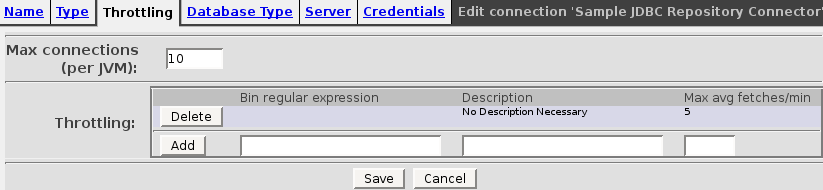
\includegraphics[width=300pt]{JDBC-edit-repository-tab3}

\begin{itemize}

\item \textbf{Max connections (per JVM):} Here you can set the maximum
number of connections to your repository.  \ifCombinedConnectorGuide
The maximum number of connections per JVM is important for three
reasons; licensing, appliance resources, and the possiblity of
overwhelming the ingestion interface. For a more complete explanation,
see the Max Connections item on page \pageref{maxrepocon}.\fi

\ifJDBCGuide
The maximum number of connections per JVM is important for three reasons.
First, the number of connections may impact the licensing on your document
server, depending on the repository.

Second, the number of connections may impact the resources
available on the appliance. If the connector framework is slowing down
your appliance, lowering this number should help.

Third, only ten document streams can be processed by the appliance
at one time.  If you are also using other repository connectors or
the \command{ingest} command on the appliance, you should reduce this
number to prevent contention for the Ingestion interface. The JDBC
Connector will never overwhelm the interface on its own, but when other
applications are also using the ingestion interface, it may be best to
set the number of repository connections to five or even fewer.
\fi


\item \textbf{Throttling:} Here you can set a maximum document fetch
rate for the repository connection.

The maximum fetch rate allows you to set three things: Expression,
description, and fetches per minute. Expression allows you to provide
a regular expression to match against document bins.  Each document
ingested through a connector is associated with one or more document
bins. These bins represent the servers that the connector interacts
with to obtain the document.  Typically, a document will be associated
with only one document bin, representing the repository server hosting
the document. For some repository connections, documents ingested
through the connector can be hosted by different servers. In the JDBC
Connector, documents only come from one server, which you will set on
the ``Server'' tab. Simply leave the expression blank; this will match
any server you enter on the ``Server'' tab.  All you need to set is
the number of document fetches per minute.  Description is an optional
field that allows you to provide a short text description of the
throttle.  Once you have set the fetch rate and optional description,
click Add.


\end{itemize}

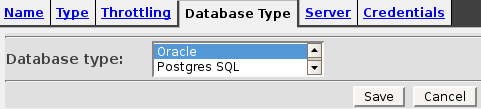
\includegraphics[width=300pt]{JDBC-edit-repository-tab4}

\begin{itemize}

\item \textbf{Database Type:} Here you should select the type of
database to which you are connecting. Currently supported databases
include Oracle, Postgres SQL, MS SQL Server (Version greater than
6.5), and Sybase (Version 10 and greater).

\end{itemize}

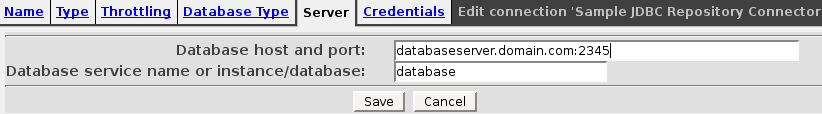
\includegraphics[width=300pt]{JDBC-edit-repository-tab5}

\begin{itemize}

\item \textbf{Server Database Host and Port:} Ask your database
administrator to provide you with the correct host name and port
number for your repository. This should be of the form
\url{databaseserver.domain.com:port}.

\item \textbf{Database service name or instance/database:} This should
be the name of the database you wish to crawl in the form
\command{database} or \linebreak \command{instance/database}.

\end{itemize}

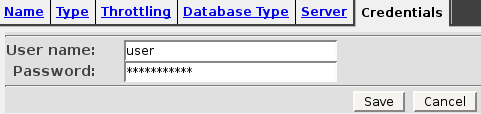
\includegraphics[width=300pt]{JDBC-edit-repository-tab6}

\begin{itemize}

\item \textbf{Name:} This is the username that the GTS appliance will
use to connect to your database server. It is recommended that the GTS
appliance be given its own username in the system. The appliance will
need to be granted appropriate permissions to select from the tables
you wish to crawl.

\item \textbf{Password:} This is the password that corresponds to the
username provided above.

\end{itemize}


After entering this information, you will be taken to the repository 
connection status page for this repository:

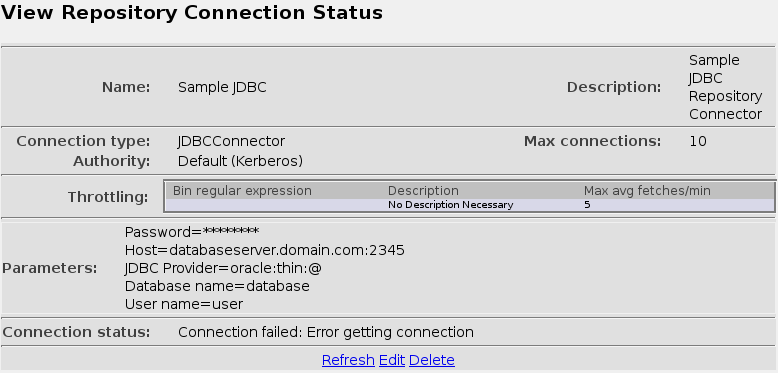
\includegraphics[width=300pt]{JDBC-view-repo-conn-status}

In this example (which does not contain accurate information for any
JDBC Connector), the Connection Status is ``Connection failed.''
If you see this message, you most likely have incorrectly entered one
of the fields, and should click ``Edit'' to fix the data. If you have
entered everything as you intended, please inform your database administrator;
you may not have been given the correct information.
